\chapter{\textit{Data Warehousing} (DWing)} 

Os principais fatores para a adoção de um programa de métricas em 
organizações de desenvolvimento de software são\begin{inparaenum}[i)]
\item a regularidade da coleta de dados;
\item a utilização de uma metodologia eficiente e transparente nessa coleta; 
\item o uso de ferramentas (não-intrusivas) para automatizar a coleta; 
\item o uso de mecanismos de comunicação de resultados adequados para todos os envolvidos; 
\item o uso de sofisticadas técnicas de análise de dados;
\apud{Gopal2005}{Silveira2010}.
\end{inparaenum} 


\textit{Data Warehousing} (DWing) é uma coleção de tecnologias de suporte à decisão disposta a capacitar os reponsáveis por tomar decisões a fazê-las de forma mais rápida \apud{chaudhuri1997}{andre2000}. Em outras palavras, trata-se de um processo para montar e gerenciar dados vindos de várias fontes, com o objetivo de prover uma visão analítica de parte ou todo o negócio \cite{gardner1998}. Desta forma, é possível em um ambiente de \textit{data warehousing} que as métricas de código-fonte sejam coletadas de fontes diversas em uma periodicidade definida, de forma automatizada, não intrusiva ao trabalho da equipe de desenvolvimento e que estas possam mostrar a qualidade total do código-fonte produzido pela equipe durante um determinado período de tempo (dias, meses, anos). 


\begin{figure}[h!]
\centering
	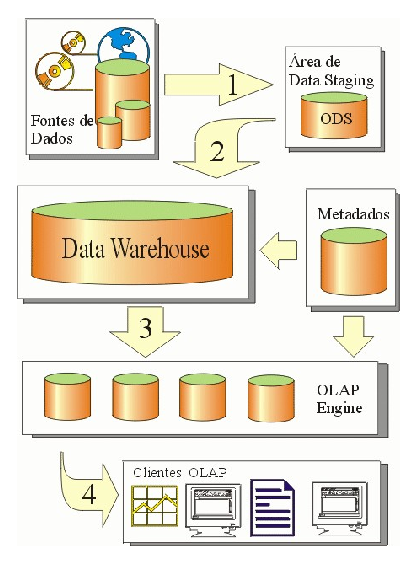
\includegraphics[keepaspectratio=true,scale=1.1]{figuras/Dwing.eps}
	\caption{Arquitetura de um ambiente de \textit{Data Warehousing} extraído de 
	\citeonline{andre2000}}
	\label{dwing}
\end{figure}
\FloatBarrier



A Figura \ref{dwing} descreve uma arquitetura geral de um ambiente de DWing, de tal forma que,

\begin{inparaenum}[i)]
	\item As setas 1 e 2 representam o processo de \textit{Extraction-Transformation-Load};
	
	\item A seta 3 representa as consultas \textit{On-Line Analytical Processing (OLAP)};
	
	\item por fim a seta 4 representa a visualização dos dados;

\end{inparaenum}
 
 	Cada um dos componentes da Figura \ref{dwing} é descrito nas seções subsequentes.



\section{\textit{Extraction-Transformation-Load} (ETL)}

As etapas de extração, transformação, carga e atualização do \textit{data
warehouse}, formam o back-end e caracterizam o processo chamado Extraction-
Transform-Load (ETL). Esse processo pode ser dividido em três etapas distintas
que somadas podem podendo consumir até 85\% de todo o esforço em um DWing
\cite{Kimball2002}.




\begin{easylist}[itemize]

& Extração: No ambiente de \textit{data warehousing}, os dados, que provêm de fontes distintas tais como planilhas, bases relacionais em diferentes tipos de
banco de dados (MySQL, Oracle, Postgres e etc) ou mesmo de web services, são inicialmente extraídos de fontes externas de dados para um ambiente de 
\textit{staging} que \citeonline{Kimball2002} considera com uma área de armazenamento intermediária entre fontes e o \textit{data warehouse}. Normalmente, é de natureza temporária e o seu conteúdo é apagado após a carga dos dados no \textit{data Warehouse}. 

& Transformação: Após os dados serem carregados na área de \textit{staging}, 
os dados passam por processos de transformações diversas. Estas podem envolver
desde uma simples transformação de ponto para vírgula, até a realização de cálculos, como por exemplo, cálculos estatísticos. 


& Carga: Após as devidas transformações dos dados, os dados são carregados, em formato pré-definido pelo projeto do \textit{data Warehouse},  em definitivo no afim de serem utilizados pelas consultas OLAP. 

\end{easylist}
 
\section{\textit{Data Warehouse}} 

\textit{Data Warehouse} (DW) é um conjunto de dados integrados, consolidados,históricos, segmentados por assunto, não-voláteis, variáveis em relação ao tempo, e de apoio às decisões gerenciais \cite{Inmon1992}, ou seja, trata-se de um repositório central e consolidado que se soma ao conjunto de tecnologias que compõem um ambiente maior, que é o DWing \cite{Kimball2002}. 


A necessidade de centralização e agregação dos dados em um \textit{data warehouse} mostrou que a modelagem relacional com a utilização das técnicas de normalização, que visam a eliminação da redundância de dados, não é eficiente quando se realiza consultas mais complexas que fazem uso frequente da operação JOIN entre várias tabelas, pois oneram recursos hardware com grandes quantidades de acesso físico a dados. \cite{Kimball2002}

Dado esse cenário, \citeonline{Kimball2002} propôs que o \textit{data warehouse} deve ser projetado de acordo com as técnicas de modelagem dimensional, que visam exibir os dados em níveis adequados de detalhes e otimizar consultas complexas \cite{valeria2012}. No modelo dimensional, são aceitos que as tabelas possuam redundância e esparcidade de dados e estas podem ser classificadas em tabelas fatos e tabelas dimensões. Estas contém dados textuais, que pode conter vários atributos descritivos que expressam relações hierarquizáveis do negócio. Já uma tabela fato é uma tabela primária no modelo dimensional onde os valores númericos ou medidas do negócio são armazenados \cite{Kimball2002}.


Assim quando se juntam fatos e dimensões, obtém-se o chamado esquema estrela, tal como se mostra na Figura \ref{estrela}. Quando os registros de uma tabela fato, podem ser somados a qualquer dimensão, é dito que o fato é aditivo. Quando é possível apenas somar em relação a algumas dimensões, é dito que o fato é semiaditivo. Já quando o fato é usado apenas para registro e não pode ser somado em relação a nenhuma dimensão, é dito que o fato é não aditivo \cite{Inmon1992}.


\begin{figure}[h!]
\centering
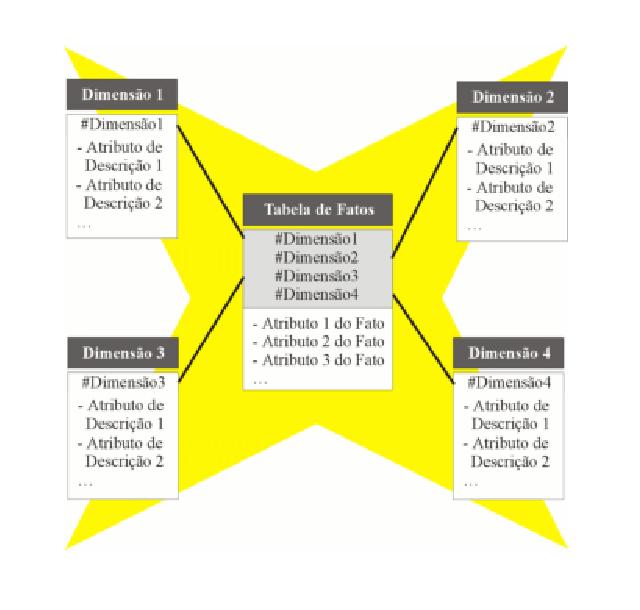
\includegraphics[keepaspectratio=false,scale=1]{figuras/estrela.eps}
\caption{Exemplo de Esquema Estrela extraído de \citeonline{andre2000}}
\label{estrela}
\end{figure}
\FloatBarrier


No esquema da Figura \ref{estrela}, percebe-se que uma tabela fato expressa um relacionamento muitos para muitos com as tabelas dimensões, mostrando assim que a navegabilidade dos dados quantitativos e qualitativos é mais intuitiva quando comparada com o modelo relacional normalizado \cite{Kimball2002}. Além disso, verifica-se que a tabela fato possui uma dimensão temporal associada, isto é, há fatos que ocorrem diariamente, como por exemplo, a venda de produtos em um supermercado. Contudo, é possível que as vendas sejam vistas por visões mensais, trimestrais, semestrais ou anuais. Logo, a granuladidade dos fatos é deve ser considerada na hora de projetar um \textit{data warehouse}.




\section{\textit{On-Line Analytical Processing} (OLAP)}

O termo OLAP, inicialmente proposto por \citeonline{Codd1993}, é utilizado para caracterizar as operações de consulta e análise em um \textit{data warehouse} projetado sobre um modelo dimensional \cite{Kimball2002}. Isto permite consultas mais flexíveis quando comparadas com as consultas \textit{Online Transaction Processing} (OTLP) que são executadas em bancos dados relacionais normalizados  visando a eliminação da redudância de dados.

As principais diferenças das operações \textit{On-Line Analytical Processing} (OLAP) para as operações 
\textit{Online Transaction Processing} (OTLP) são apresentados na Tabela 
\ref{olapxoltp}.

	\begin{table}[!ht]
	\begin{center}
	 \begin{tabular}{|p{5cm}|p{5cm}|}
		\hline
		OLAP & OLTP \\ \hline
		Modelagem Dimensional (Tabelas Fato e Dimensão) & Modelagem Relacional com a utilização das formas normais (3N, 4N, 5N) \\ \hline
		Dados armazenados em nível transacional e agregado    & Dados em nível em nível transacional        \\ \hline
		Visa o diminuir o uso do JOIN & Faz uso constante de Join   \\ \hline
		Estrutura de tipicamente estática   & Estrutura tipicamente dinâmica      \\ \hline
		Proveem informações atuais e do passado & Geralmente sem suporte a estado temporal dos dados
		      \\ \hline
		\end{tabular}
		\caption{Diferenças entre OLAP e OLTP extraído de \citeonline{valeria2012} e \citeonline{andre2000}}
		\label{olapxoltp}
		\end{center}
		\end{table}

As operações OLAP tem como objetivo prover visualização dos dados sob diferentes perspectivas gerenciais e comportar todas as atividades de análise. Estas podem ser feitas de maneira \textit{ad hoc}, por meio das ferramentas de suporte à operações OLAP. Contudo, há algumas, que são documentadas pela literatura, e são classificadas em dois grupos: Análise Prospectiva e Análise Seletiva \apud{chaudhuri1997}{andre2000}.

A análise prospectiva consiste em realizar a análise a partir de um conjunto inicial de dados para chegar a dados mais detalhados ou menos detalhados \cite{Inmon1992}. Já a análise seletiva tem como objetivo trazer à evidência para os dados \cite{andre2000}. Entre as operações de análise prospectiva estão:

\begin{easylist}[itemize]

& \textit{Drill-Down}: Descer no nível de detalhes dos dados de uma dimensão. isto é,  adicionar cabeçalhos de linha de tabelas de dimensão \cite{Kimball2002}

& \textit{Roll-Up}: contrário de Drill-Down, trata-se caminhar para a visão de dados mais agregados \apud{Kimball2002}{andre2000}. 

& Drill-Across: significa caminhar a partir de uma dimensão para
outra dimensão, combinando-as para mudar o enfoque da
análise \cite{andre2000}.

\end{easylist}

Entre as operações de análise seletiva estão:

\begin{easylist}[itemize]

& \textit{Slice and Dice} : Em português, significa cortar e fatiar. Esta operação seleciona pedaços transversais do modelo dimensional e em seguida aplica critérios de seleção sobre este pedaço. \cite{andre2000}. Ou seja trata-se de uma operação semelhante a clásula WHERE do SQL \cite{valeria2012}

& \textit{Pivoting} : Trata-se de uma operação de rotação, isto é, muda-se a orientação das tabelas dimensionais afim de restrigir a visualização de dimensões em um relatório. \cite{andre2000}.

\end{easylist}

\section {Visualização de Dados}

\section{Metodologia do Projeto do \textit{Data Warehouse}}

\citeonline{Kimball2002} enuncia que o ambiente de DWing nasce na necessidade do negócio e logo o projeto de um \textit{data warehouse} deve seguir os seguintes passos: 

\begin{inparaenum}[1)]
	\item Selecionar o Processo de Negócio com requisito fundamental do 
	projeto DW;
	
	\item Declarar a granularidade dos dados necessários para processo de 
	negócio, isto é, verificar a periodicidade de coleta dos dados (diários, semanais, mensais, trimestrais, semestrais ou anuais);
	
	\item Escolher as dimensões;
	
	\item Identificar os fatos;

\end{inparaenum} 


Seguindo a metolodogia proposta por \citeonline{Kimball2002}, entendeu-se que o processo de negócio, neste trabalho de conclusão de curso, foi avaliar a qualidade do código-fonte continuamente por meio das métricas de código-fonte.
Os demais passos da metodologia, tais como, a granulidade dos dados, identificação dos fatos e dimensões são apresentados no Capítulo \ref{estudo de caso}.


